\documentclass{beamer}
\usepackage[italian]{babel}
%\usepackage[latin1]{inputenc}
\usepackage[T1]{fontenc}
%%%%%%%%%%%%%%%%%%%%%%%%%
%\usepackage{color}
%\usepackage{amsmath}
%\usepackage{minted}
%\usepackage[italian]{babel}
%\usepackage{graphics}
%\usepackage{graphicx}
%\usepackage[subfigure]{}
%\usepackage{setspace}
\usepackage[utf8]{inputenc}%
%%%%%%%%%%%%%%%%%%%%%%%%%





\title{Metodologie e tecniche di Continuous Integration per l'evoluzione di OpenStack}

%\author[Euclide]{Euclide di Alessandria \\
%\texttt{euclide@alessandria.edu}}
%\date[VII SINP]{VII Simposio Internazionale sui Numeri Primi}

\author[A.Copler e L.Calomeni]{
  Alessandro Copler\\
  \texttt{alessandro.copler@gmail.com}\\
  \and
  Luca Calomeni\\
  \texttt{lcalomeni@gmail.com}
}


\institute[UniDiBergamo]{Università degli studi di Bergamo - Facolta di Ingegneria}
%\logo{
\includegraphics[width=3cm]{unibg.jpg}}

\usetheme{Hannover}
%\usecolortheme{spruce}
%\usetheme{AnnArbor}
%\useoutertheme[right]{sidebar}
\setbeamercovered{dynamic}
\theoremstyle{definition}
\newtheorem{definizione}{Definizione}
\theoremstyle{plain}
\newtheorem{teorema}{Teorema}
\newtheorem{obiettivo}{Obiettivo}
\newtheorem{obiettivi}{Obiettivi}
\newtheorem{vantaggi}{Vantaggi}
\newtheorem{svantaggi}{Svantaggi}
\newtheorem{clonazione_full}{Clonazione Full}
\newtheorem{clonazione_linked}{Clonazione Linked}
\begin{document}
\begin{frame}
\maketitle
\end{frame}


\begin{frame}
\frametitle{Piano della presentazione}
\tableofcontents
\end{frame}

\section{Introduzione}

\subsection{Cloud
Computing}

%\begin{frame}
%\frametitle{Using Columns}
%\begin{columns}
%\column{0.5\textwidth}
%<text>
%\column{0.5\textwidth}
%<text>
%\end{columns}
%\end{frame}


\begin{frame}
\frametitle{Che cos'è il Cloud Computing?}
%cos'è
%pubblico privato ecc
\begin{definizione}

Il \alert{Cloud Computing} è un gruppo distribuito di server interconnessi che gestiscono servizi, eseguono applicazioni ed archiviano documenti con la totale predisposizione alla scalabilità rispetto all'utilizzo richiesto.
\end{definizione}
\begin{columns}
\column{0.5\textwidth}
Tipologia dei servizi:
\begin{itemize}
\item
PaaS
\item
IaaS
\item
SaaS
\end{itemize}
\column{0.5\textwidth}
\begin{figure}[!h]
	\begin{center}

\includegraphics[width=3cm]{cloud.png}
\end{center}
\end{figure}

\end{columns}

\end{frame}

\begin{frame}
\frametitle{Tipi di Cloud}
\begin{itemize}
\item
Pubblico
\item
Privato
\item
Ibrido
\item
Community
\end{itemize}
\end{frame}
%%%%%%%%%%%%%%%%%%%%%%%%%%%%%%%%%%%%%%%%%%%%%%%%%%%%%%%%%%%%%%%%%%%%%%5
\subsection{OpenStack}
\begin{frame}
\frametitle{Che cos'è OpenStack?}
\begin{definizione}
\alert{OpenStack} è un software open-source che fornisce un'infrastruttura cloud modulare, in grado di offrire servizi di gestione di processi e storage secondo il modello IaaS.

\begin{figure}[!h]
	\begin{center}

\includegraphics[width=3cm]{openstack.png}
\end{center}
\end{figure}

\end{definizione}
\end{frame}


\begin{frame}
\frametitle{Il progetto Escudo-Cloud}
\alert{Escudo-Cloud} è un progetto europeo nato dalla collaborazione di diversi partner industriali internazionali come IBM e British Telecom e accademici come l'\textbf{Università degli studi di Bergamo} e l'Università degli studi di Milano.\\
\vspace*{1cm}
\begin{columns}
\column{0.8\textwidth}
\begin{obiettivi}
\begin{itemize}
\item
tecniche e metodi per la gestione delle chiavi
\item
protezione data-at-rest
\item
fornire un layer di protezione tra client e provider
\end{itemize}
\end{obiettivi}
\column{0.2\textwidth}
\begin{figure}[!h]
	\begin{center}

\includegraphics[width=1.5cm]{ESCUDO-CLOUD.png}
\end{center}
\end{figure}
\end{columns}
\end{frame}
%%%%%%%%%%%%%%%%%%%%%%%%%%%%%%%%%%%%%%%%%%%%%%%%%%%%%%%%%%%%%%%%%%%%%%%%%%%%
\subsection{Continuous Integration con Jenkins}
\begin{frame}
\frametitle{Cosa si intende per Continuous Integration?}
\begin{definizione}
La \alert{Continuous Integration} una pratica di sviluppo software dove i membri di un team \alert{integrano} il proprio lavoro \alert{frequentemente}.
\end{definizione}
\vspace*{0.5cm}
Ogni integrazione deve essere \alert{verificata} da una build automatizzata e \alert{testata}.
\begin{obiettivo}
Individuare errori di integrazione il più presto possibile.
\end{obiettivo}

\end{frame}


\begin{frame}
\frametitle{Jenkins per la Continuous Integration}
\begin{definizione}
\alert{Jenkins} è uno strumento di Continuous Integration open source scritto in Java
\end{definizione}
\begin{columns}
\column{0.5\textwidth}
\begin{vantaggi}
\begin{itemize}
\item
interfaccia utente user friendly
\item
potente e estensibile con plugin
\item
comunità solida e numerosa
\end{itemize}
\end{vantaggi}
\column{0.5\textwidth}
\begin{svantaggi}
\begin{itemize}
\item
a\\
a
\item
a\\
a
\item
a\\
a
\end{itemize}
\end{svantaggi}
\end{columns}
\end{frame}
%%%%%%%%%%%%%%%%%%%%%%%%%%%%%%%%%%%%%%%%%%%%%%%%%%%%%%%%%%%%%%%%%%%%%%%%%%%%

\section{Stato dell'arte}
\subsection{Processo di validazione della Fondazione OpenStack}
\begin{frame}
\frametitle{Come si contribuisce OpenStack}
\begin{figure}[!h]
	\begin{center}
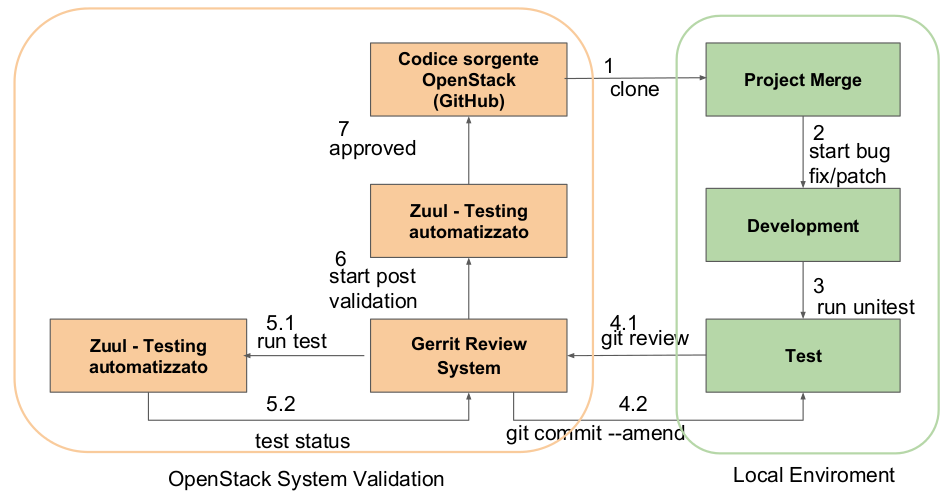
\includegraphics[width=10cm, height=7cm]{sviluppo.png}
%	\caption{Processo di sviluppo e validazione}
%	\label{fig:pre_processo_sviluppo_validazione}
\end{center}
\end{figure}
\end{frame}



%%%%%%%%%%%%%%%%%%%%%%%%%%%%%%%%%%%%%%%%%%%%%%%%%%%%%%
\section{Configurazioni studiate}
\subsection{Come varia il processo}
\begin{frame}
\frametitle{Come varia il processo}
\begin{figure}[!h]
	\begin{center}
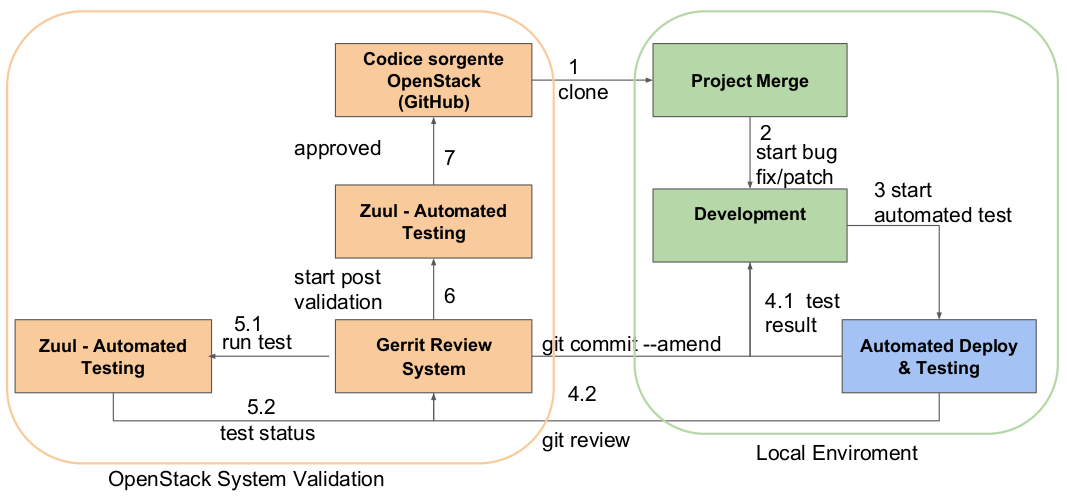
\includegraphics[width=10cm, height=7cm]{sviluppo_ci.png}
%	\caption{Processo di sviluppo e validazione}
%	\label{fig:pre_processo_sviluppo_validazione}
\end{center}
\end{figure}
\end{frame}

\begin{frame}
\frametitle{Come varia il processo}
\begin{figure}[!h]
	\begin{center}
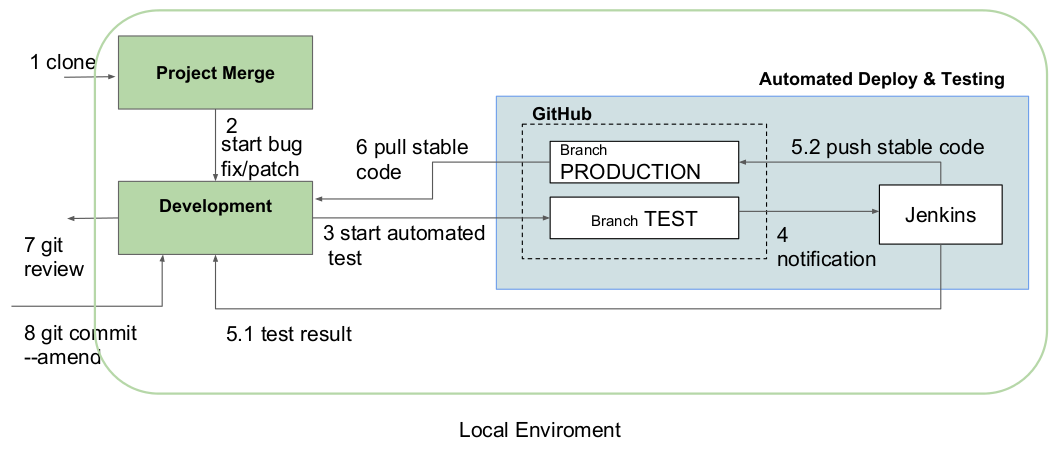
\includegraphics[width=10cm, height=6cm]{schema_alto_livello.png}
%	\caption{Processo di sviluppo e validazione}
%	\label{fig:pre_processo_sviluppo_validazione}
\end{center}
\end{figure}
\end{frame}



\subsection{Prima configurazione con singolo progetto}
\begin{frame}
\frametitle{Configurazione singolo progetto}
\begin{figure}[!h]
	\begin{center}
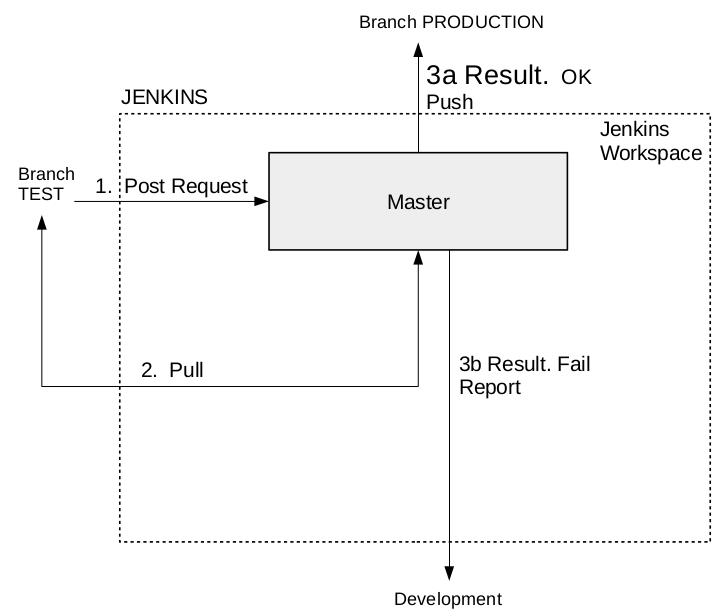
\includegraphics[width=10cm, height=6cm]{conf1.png}
%	\caption{Processo di sviluppo e validazione}
%	\label{fig:pre_processo_sviluppo_validazione}
\end{center}
\end{figure}
\end{frame}

\subsection{Seconda configurazione con multi progetti}
\begin{frame}
\frametitle{Configurazione multi progetto}
\begin{figure}[!h]
	\begin{center}
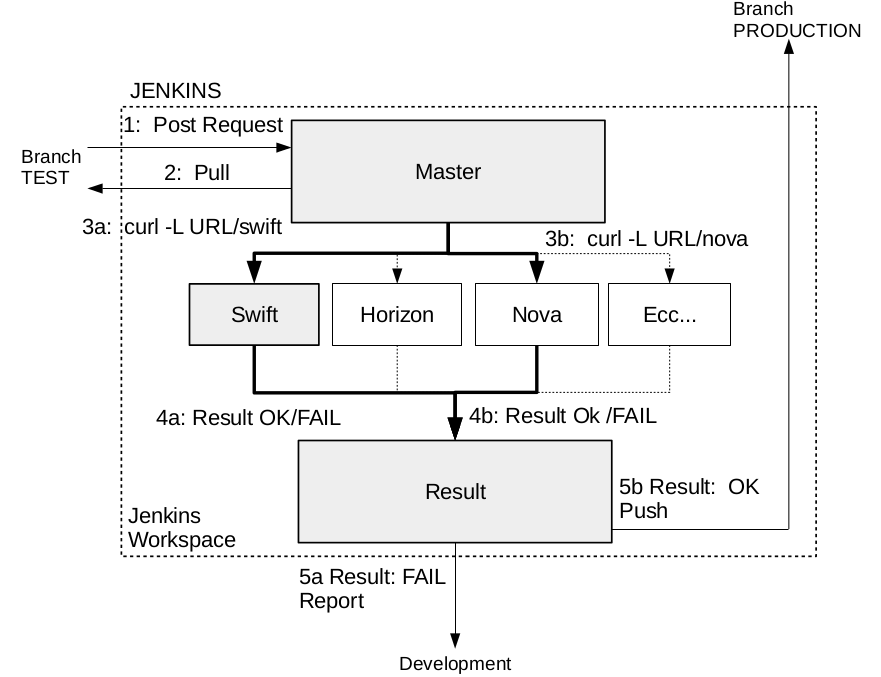
\includegraphics[width=10cm, height=7cm]{conf2.png}
%	\caption{Processo di sviluppo e validazione}
%	\label{fig:pre_processo_sviluppo_validazione}
\end{center}
\end{figure}
\end{frame}

\begin{frame}
\frametitle{Configurazione multi progetto}
\begin{columns}
\column{0.5\textwidth}
\begin{clonazione_full}
\begin{itemize}
\item
copia totale della macchina virtuale
\item
\textcolor{green}{macchina clonata indipendente}
\item
spazio occupato doppio
\item
tempo clonazione considerevole
\end{itemize}
\end{clonazione_full}
\column{0.5\textwidth}
\begin{clonazione_linked}
\begin{itemize}
\item
copia parziale legata alla macchina originale
\item
macchina clonata collegata 
\item
\textcolor{green}{spazio occupato scalabile}
\item
\textcolor{green}{tempo clonazione irrilevante}
\end{itemize}
\end{clonazione_linked}
\end{columns}
\end{frame}

\subsection{Terza configurazione multi progetti indipendenti}
\begin{frame}
\frametitle{Configurazione multi progetti indipendenti}
\begin{figure}[!h]
	\begin{center}
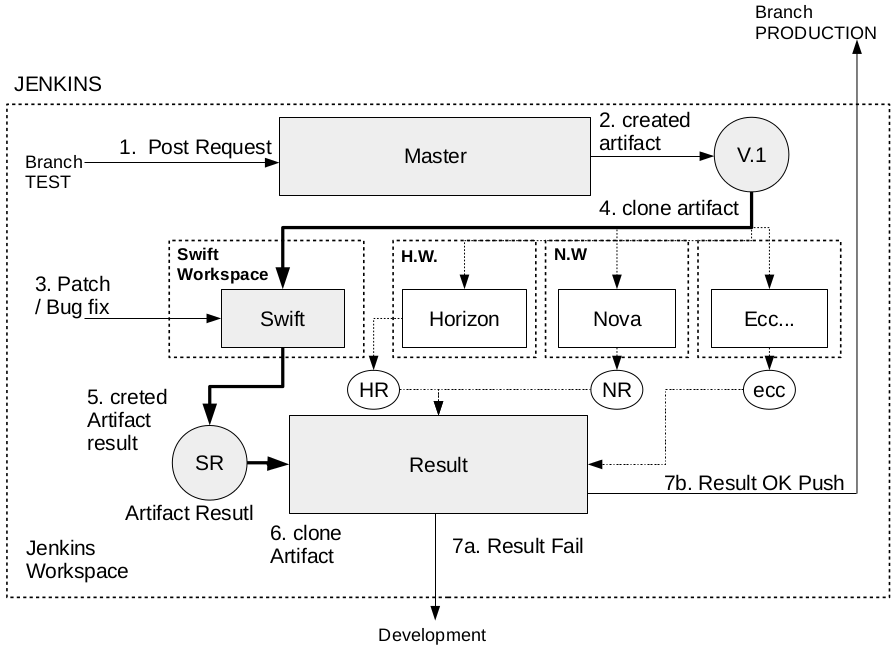
\includegraphics[width=10cm, height=7cm]{conf3.png}
%	\caption{Processo di sviluppo e validazione}
%	\label{fig:pre_processo_sviluppo_validazione}
\end{center}
\end{figure}
\end{frame}



\begin{frame}
\frametitle{Configurazione multi progetti indipendenti}
\begin{definizione}
\alert{Artifact} bla bla
\end{definizione}
\end{frame}

\section{Benchmark dei risultati}

\subsection{Benchmark}
\begin{frame}
\frametitle{Benchmark dei tempi medi ottenuti}
\begin{definizione}
 \alert{benchmark} bla bla
\end{definizione}
\end{frame}

\subsection{Trade-off}
\begin{frame}
\frametitle{Trade-off performance}
\begin{definizione}
\alert{trade-off} bla bla
\end{definizione}
\end{frame}

\section{Considerazioni finali e possibili sviluppi futuri}
\subsection{Commenti finali}
\begin{frame}
\frametitle{Che cosa sono i numeri primi?}
\begin{definizione}
Un \alert{numero primo} è un intero $>1$ che ha esattamente
due divisori positivi.
\end{definizione}
\end{frame}
\subsection{Sviluppi futuri}
\subsection{Ringraziamenti}
\end{document}